\documentclass{article}

\usepackage{graphicx}
\usepackage{amssymb}
\usepackage[utf8]{inputenc}
\usepackage[T1]{fontenc}

\renewcommand{\familydefault}{\sfdefault}
\usepackage[scaled=1]{helvet}
\usepackage[helvet]{sfmath}
\everymath={\sf}

\title{Reporte de Actividad 2}

\author{Diego Iván Moreno Campa}

\date{2 de Febrero, 2018}

\begin{document}

\maketitle

\bigskip

\section{Introducción}

Esta actividad es el segundo trabajo para la materia de Física computacional I en la licenciatura de Física.

El propósito de la actividad es familiarizarse con el entorno de Jupyter para escribir en lenguaje Python, el cual tiene numerosas funciones; estudiaremos las bibliotecas de Python para realizar cálculos numéricos Numpy y manejo de datos Pandas. La forma en que usaremos Python es para manejar datos de las estaciones en localidades Mexicanas.

\section{Inicializando el entorno de desarrollo}

Para empezar a utilizar Python tenemos que abrir el entorno en el que trabajaremos, Jupyter, por lo tanto, comenzamos abriendo una terminal localizada en el espacio de trabajo de nuestro ordenador y después ejecutamos el comando "\textit{Jupyter Notebook}" en la terminal para iniciar el servidor de Jupyter en el directorio local y comenzar a escribr en la plataforma.

\section{Búsqueda de datos}

Para comenzar a practicar con Python, es necesario tener unos datos a manejar, es por eso que buscamos datos en la página que se nos proporcionó, donde se pueden encontrar los datos sobre el entorno de alguna posición de lectura del ambiente en México: "http://smn1.conagua.gob.mx/emas/". ~\\
\indent Personalmente elegí nogales no solo porque esta cerca de casa sino porque también de los que había elegido anteriormente fue uno de los únicos que tenia datos limpios, consistentes y sin renglones vacíos.

En el documento de datos sobre el entorno 

\section{El Documento}

Para crear el documento donde escribiremos el código en Python, se necesita crear una libreta en Jupyter entrando a la plataforma y seleccionando el listado desplegable "\textit{New $\blacktriangledown$}" y seleccionando la opción Python 3.0. El profesor nos proporcionó con un ejemplo para la organización de datos en Python dentro de su repositorio en GitHub.

\subsection{Declarando Paquetes}

La primera celda que utilizamos fue la declaración de paquetes para el archivo de Python, donde se declararon los siguientes paquetes:
\begin{itemize}
\item Pandas: Una librería que provee herramientas de alto rendimiento al analizar y estructurar datos para el lenguaje de programación Python.
\item NumPy: Una librería para el lenguaje de programación Python, que añade soporte a arreglos y matríces multidimensionales de numeros grandes, así como también se proporciona una gran colección de funciones matemáticas de alto nivel para operar en estos arreglos.
\item MatplotLib: Una librería para generar gráficas en Python
\end{itemize}

Los cuales se declararon como se muestra a continuación, con nombres cortos para después ser llamados ágilmente.
\begin{figure}[h]
\centering
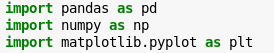
\includegraphics[height=27px,width=137px]{1stcell.png}
\end{figure}

Para ejecutar una celda dentro del entorno Jupyter se utiliza el comando de teclado "\textit{Shift$+$Enter}"

%\begin{wrapfigure}{l}{0.5\textwidth}
%   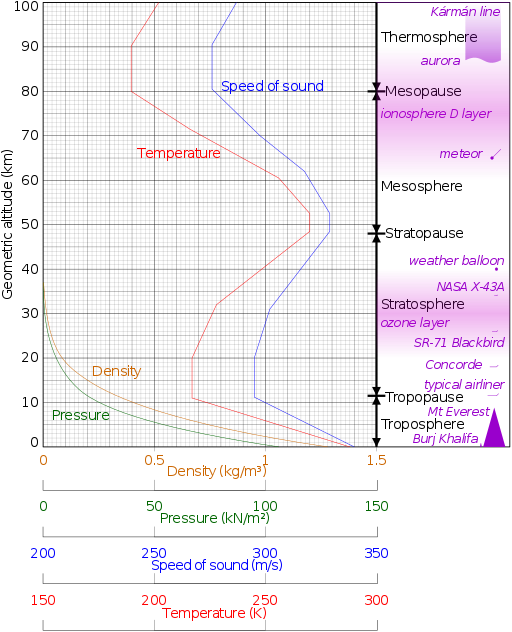
\includegraphics[height=5cm,width=0.50\textwidth]{AtmosModel.png}
%	\caption{Comparación de la gráfica de la atmósfera estandar Estadounidense de altitud gráfica contra presión, densidad, temperatura y velocidad del sonido, junto a alturas aproximadas de varios objetos.}
%\end{wrapfigure}

\newpage

\subsection{Entrada de datos}

Continuamos en la siguiente celda introduciendo los datos de la hoja de texto con los datos del entorno de Nogales. Para esto declaramos una variable, en este caso llamada df0, que tomara los valores de la hoja de texto que le especifiquemos a través una función proporcionada por Pandas para leer archivos y traerlos a DataFrame, "read\_ csv()". Se especificó la dirección del archivo que se lee, después se agregó un atributo para saltarse las primeras 4 filas, las cuales no contienen ningún dato manejable, y se agregó el atributo "sep='\textbackslash s+'" para leer los datos con más de un espacio entre columnas.
\begin{figure}[h]
\centering
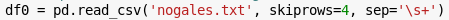
\includegraphics[height=10px,width=224px]{2ndcell.png}
\end{figure}



\subsection{Leer encabezado}

Para leer el encabezado de un archivo de datos se utiliza la función head(), la cual imprime las primeras 5 filas del archivo.
\begin{figure}[h]
\centering
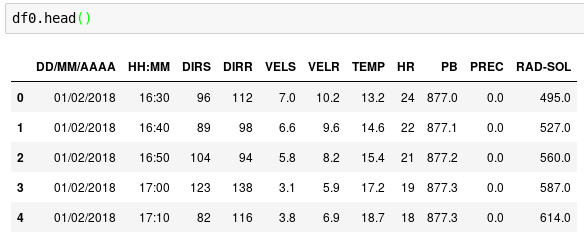
\includegraphics[height=119px,width=292px]{3rdcell.png}
\end{figure}

\subsection{Estructuramiento de datos}

En estos momentos los datos estan desorganizados y no tienen forma dentro del contexto de Python, sin embargo, para esto existe la funcion DataFrame() de Pandas, que le da una estructura al texto para que pueda ser leído por el código. Declaramos una nueva variable que contenga la función Dataframe() con el atributo df0, la variable sin estructura que declaramos al inicio, y con el nombre df para abreviar.

Después, en la siguiente celda ejecutamos una función para observar el tipo de datos que puede leer Python para cada columna de datos.
\begin{figure}[ht]
\centering
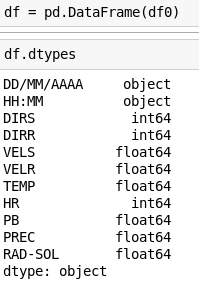
\includegraphics[height=146px,width=99px]{4th5thcell.png}
\end{figure}

\newpage

Para continuar con el estructuramiento de datos, en la siguiente celda se ejecuta una funcion sobre el DataFrame para combinar las columnas de "DD/MM/AAAA" y "HH:MM" en una sola columna llamada Fecha con el tipo Tiempo, como le sigue, se eliminan las correspondientes columnas que se combinaron. Observamos los cambios volviendo a imprimir el encabezado:
\begin{figure}[h]
\centering
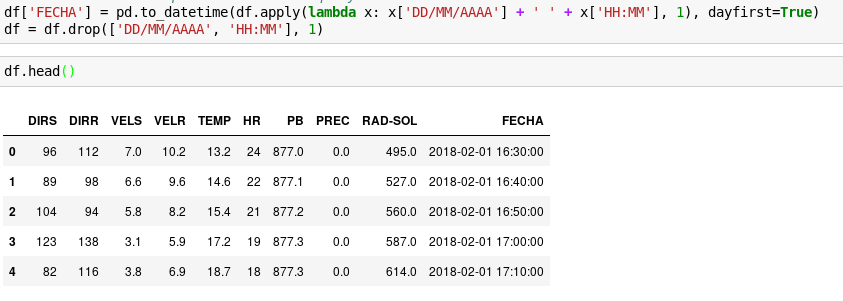
\includegraphics[height=150px,width=421px]{6th7thcell.png}
\end{figure}

\subsection{Resumen y selección de datos}

Siempre que tenemos un listado o arreglo de datos es importante conocer los aspectos característicos de estos, como el promedio, la desviación y demás. En Python existe una función, describe(), para realizar esto sobre DataFrames, una función que imprime un resumen de dichas características del dataframe donde se utiliza. Esta función solo utiliza, claro está, tipos numéricos y no objetos como la fecha o la hora.
\begin{figure}[ht]
\centering
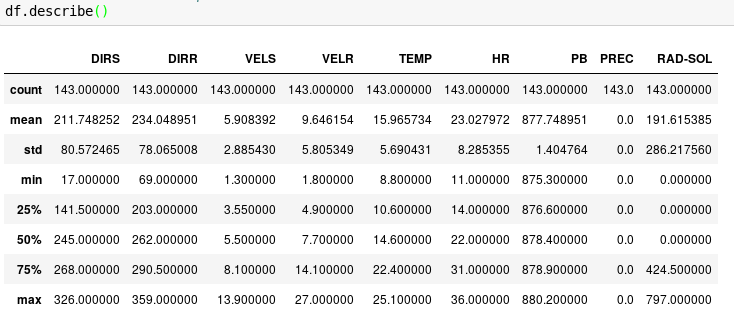
\includegraphics[height=131px,width=300px]{8thcell.png}
\end{figure}

Es importante para el manejo de datos el tener una forma de seleccionar un intervalo de datos requeridos o deseados, no utilizamos una función explicita para realizar esto, sin embargo, se realizó fácilmente al declarar algunas variables que solo tomaban un intervalo temperatura de df.
\begin{figure}[h]
\centering
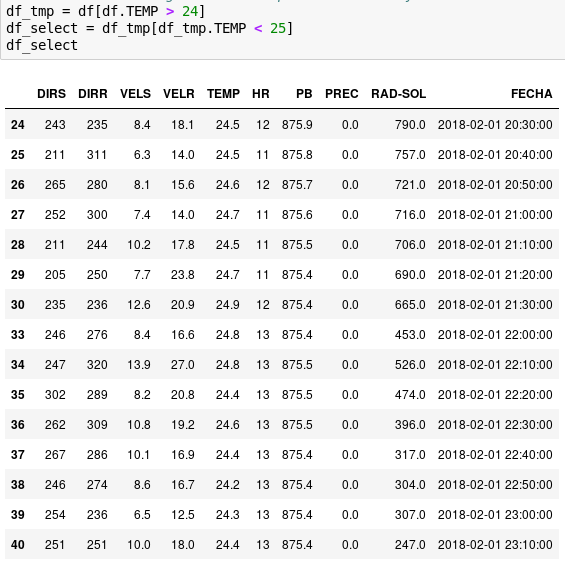
\includegraphics[height=237px,width=238px]{9thcell.png}
\end{figure}

Luego, si se desea únicamente conocer cierta característica estadística de los valores dados podemos usar ciertas funciones sobre el listado de datos, por ejemplo la funcion mean() que se puede usar sobre el DataFrame que tenemos, df. Y si deseamos obtener esta característica para una sola columna de datos entonces se especifíca ésta para mostrar únicamente este valor.
\begin{figure}[ht]
\centering
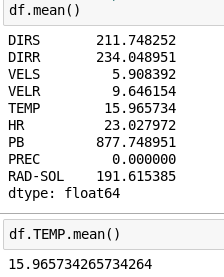
\includegraphics[height=138px,width=112px]{10th11thcell.png}
\end{figure}

\subsection{Trazado de gráficas}

Ahora podemos empezar a graficar nuestros datos estructurados, para esto primero llamamos a matplotlib \textit{plt}, usando la función figure() para crear un objeto, este sera una gráfica de la rapidez de los vientos tomada de nuestra estructura de datos \textit{df}. Después le agregamos el título, la etiqueta del "eje y", le agregamos la cuadrícula y se imprime con la funcion show().
\begin{figure}[h]
\centering
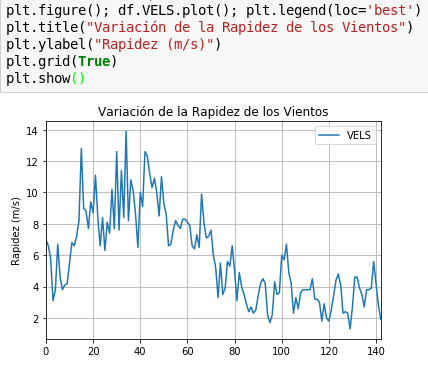
\includegraphics[height=182px,width=214px]{12thcell.png}
\end{figure}

La siguiente gráfica que se realizó consistió en presentar dos columnas de datos en una sola gráfica, a modo de comparación. Esta vez como utilizaremos más de una columna de datos es mejor especifícar en otra variable las columnas de datos que tomaremos, por ejemplo como se realiza con la variable \textit{df1}.
\begin{figure}[ht]
\centering
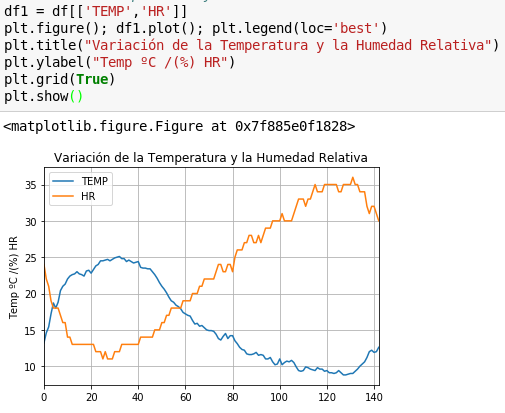
\includegraphics[height=206px,width=252px]{13thcell.png}
\end{figure}

También podemos graficar alguna relación entre dos columnas de datos asignandole a cada eje una columna de datos:
\begin{figure}[!ht]
\centering
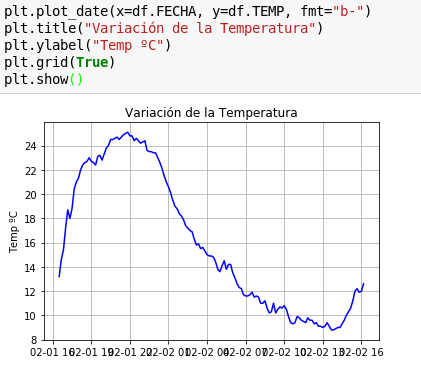
\includegraphics[height=187px,width=210px]{14thcell.png}
\end{figure}

\section{Actividades Adicionales}

En la práctica se nos pidió realizar varias actividades después de haber escrito el ejemplo del profesor.

La primera actividad consiste en crear una gráfica que muestre la rapidez de los vientos y la rapidez de las ráfagas, como funciones del tiempo. La gráfica se llevó a cabo utilizando el mismo procedimiento que se observo en el ejemplo para gráficar una columna de datos con respecto a otra:
\begin{figure}[ht]
\centering
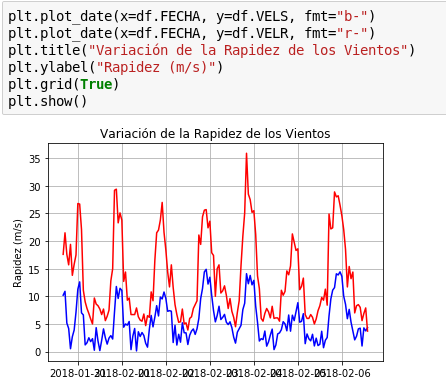
\includegraphics[height=195px,width=223px]{15thcell.png}
\end{figure}

\newpage
 
La segunda actividad consistió en crear una gráfica que muestre las direcciones, en unidades de grados, de los vientos con respecto al tiempo. Se puede notar claramente que los vientos son consistentes durante la noche hacia los 250 grados.
\begin{figure}[h]
\centering
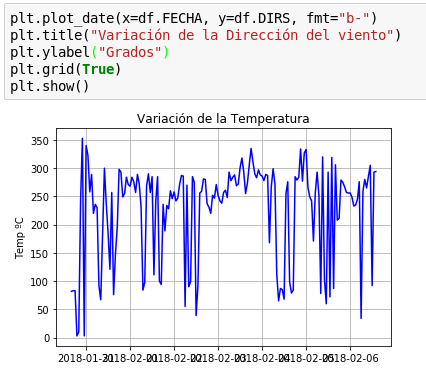
\includegraphics[height=188px,width=213px]{16thcell.png}
\end{figure}

\newpage

La tercera actividad pedia crear una gráfica que muestre la radiación solar contra el tiempo. la cual se puede notar como la radiación solar es más intensa durante el medido día como se puede asumir lógicamente.
\begin{figure}[h]
\centering
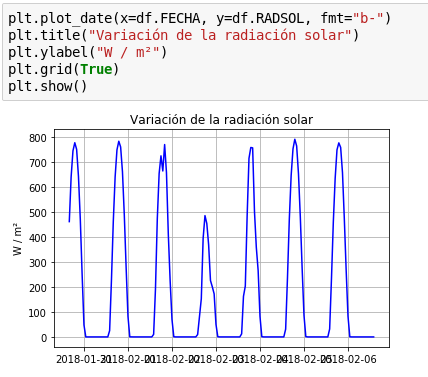
\includegraphics[height=188px,width=214px]{17thcell.png}
\end{figure}

La cuarta actividad actividad nos pide obtener el rango de temperatura diario de nuestros datos.
\begin{figure}[h]
\centering
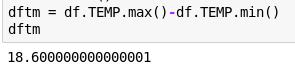
\includegraphics[height=37px,width=147px]{18thcell.png}
\end{figure}

La quinta actividad se nos pide comentar sobre la relación entre la temperatura y la humedad, la cual me parece la temperatura y la humedad son inversamente proporcional una de la otra después de observar la gráfica donde se muestran juntas. Se puede deducir pensando en el concepto microscópico de temperatura y la humedad como la concentración de moleculas de agua en el aire: entre mayor es la temperatura, mayor energía habrá en el sistema, por lo que las moleculas tendran mayores velocidades y se separaran unas de las otras, lo que hará que las moleculas de agua esten menos concentradas, esto es, habra menor humedad debido a que el agua se evapora con la temperatura.

\newpage

\section{Bibliografía}
\begin{itemize}
\item Numpy. (2018, Febrero 3) NumPy developers. Página Principal. http://www.numpy.org/
\item Pandas Python Data Analysis. (2018, Febrero 3) Python developers. Página Principal. https://pandas.pydata.org/ 
\end{itemize}

\newpage

\title{Apéndice}

\begin{enumerate}
\item ¿Cuál es tu primera impresión de Jupyter Notebook? ~\\~\\
Parece un entorno de desarrollo fácil de manejar a pesar de que no se programar en Python

\item ¿Se te dificultó leer código en Python?~\\~\\
Con mi experiencia de programador leer las funciones y variables no me pareció dificil de comprender lo que se realizaba excepto en algunos casos, y me parece que no a muchos se les dificulto esta parte

\item ¿En base a tu experiencia de programación en Fortran, que te parece el entorno de trabajar en Python? ~\\~\\
De alguna manera me parece más fácil a la hora de organizar datos, sin embargo, como esta práctica no nos llevo muy a fondo al cálculo de tipos numéricos me parece dificil comparar ambos lenguajes en este aspecto

\item A diferencia de Fortran, ahora se producen las gráficas utilizando la biblioteca Matplotlib. ¿Cómo fue tu experiencia?. ~\\~\\
Tener una forma directa de graficar tus datos me parece algo útil.

\item En general, ¿qué te pereció el entorno de trabajo en Python?  ~\\~\\
Me pareció que en esta práctica no se pudo apreciar la funcionalidad de Python muy bien en cuanto a otros usos. Aprender Python no me parece de mucha utilidad en estos momentos debido a que manejo relativamente bien Fortran, si Python me demuestra que puede hacer lo que Fortran de manera portatil y rápida, pues todo bien.

\item ¿Qué opinas de la actividad? ¿Estuvo compleja? ¿Mucho material nuevo? ¿Que le faltó o que le sobró? ¿Qué modificarías para mejorar?   ~\\~\\
Definitivamente mucho material nuevo, no me gusta cuando me obligan a hacer algo que no tengo la menor idea de que esta haciendo al inicio. Me gusta saber lo que mi programa hará y que puedo hacer o con que puedo hacerlo.

\item ¿Comentarios adicionales que desees compartir? ~\\
Ninguno mas de lo anterior


\end{enumerate}

\end{document}
